\documentclass[11pt,a4paper]{article}
\usepackage[margin=20mm,bottom=23mm]{geometry}
\usepackage[T1]{fontenc}
\usepackage[utf8]{inputenc}
\usepackage{lmodern}
\renewcommand{\familydefault}{\sfdefault}
\PassOptionsToPackage{obeyspaces}{url}
\usepackage{xcolor,tikz,tcolorbox,listings,enumitem,booktabs,array,fancyhdr,hyperref}
\usetikzlibrary{arrows.meta,positioning}
\definecolor{slate}{HTML}{183349}
\definecolor{blue}{HTML}{215C86}
\definecolor{teal}{HTML}{167F80}
\definecolor{pale}{HTML}{F0F5F8}
\definecolor{ink}{HTML}{273D4B}
\hypersetup{colorlinks=true,urlcolor=blue,linkcolor=blue,pdftitle={Panduan Pengguna GRIB ke CSV dan Excel},pdfauthor={grib-data-processing}}
\setlength{\parindent}{0pt}
\setlength{\parskip}{6pt}
\setlist{leftmargin=6mm,itemsep=4pt,topsep=4pt}
\pagestyle{fancy}
\fancyhf{}
\fancyhead[L]{\small\color{slate}GRIB ke CSV dan Excel}
\fancyhead[R]{\small\color{teal}Panduan Windows}
\fancyfoot[L]{\footnotesize 13 Oktober 2026}
\fancyfoot[R]{\footnotesize\thepage\ / 12}
\renewcommand{\headrulewidth}{0.4pt}
\setlength{\headheight}{14pt}
\newtcolorbox{panel}[1]{colback=pale,colframe=blue,boxrule=0.5pt,arc=2mm,left=3mm,right=3mm,top=2mm,bottom=2mm,title={#1},fonttitle=\bfseries}
\lstnewenvironment{terminal}{\lstset{basicstyle=\ttfamily\small,columns=fullflexible,keepspaces=true,showstringspaces=false,breaklines=false,backgroundcolor=\color{pale},frame=single,rulecolor=\color{pale},framesep=7pt,aboveskip=7pt,belowskip=7pt}}{}
\newcommand{\step}[2]{\par\addvspace{2mm}\noindent\textcolor{teal}{\textbf{#1.}}\ \textbf{#2}\par\nobreak}
\newcommand{\pagetitle}[3]{\clearpage{\color{teal}\small\bfseries LANGKAH #1}\par{\color{slate}\LARGE\bfseries #2}\par\vspace{2mm}#3\par\vspace{3mm}}
\newcommand{\source}[1]{{\footnotesize\color{blue}Sumber: [#1], daftar tautan di halaman 12.}\par}
\DeclareUrlCommand\code{\urlstyle{tt}}
\begin{document}
\color{ink}
{\color{teal}\small\bfseries MULAI DARI NOL}\par
{\color{slate}\Huge\bfseries GRIB menjadi\par CSV dan Excel}\par
\vspace{2mm}
{\Large Panduan untuk pengguna nonprogrammer}\par
Windows 64-bit \textbullet\ Python 3.11 \textbullet\ Pilihan bantuan AI\par
\vspace{6mm}
\par\noindent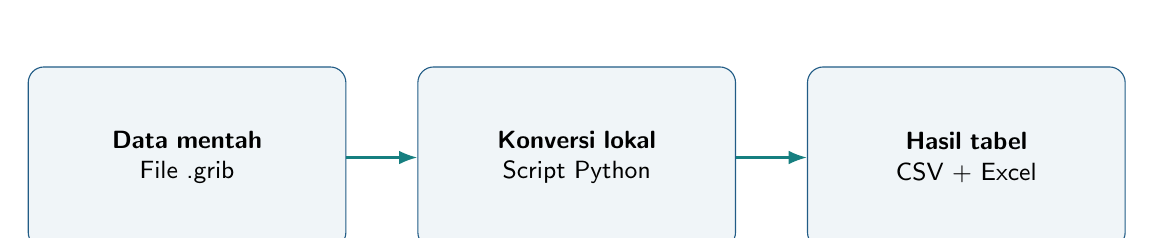
\begin{tikzpicture}[node distance=9mm,>=Latex]
\tikzset{box/.style={draw=blue,fill=pale,rounded corners=2mm,text width=38mm,minimum height=23mm,align=center,font=\small}}
\node[box] (a) {\textbf{Data mentah}\\File \code{.grib}};
\node[box,right=of a] (b) {\textbf{Konversi lokal}\\Script Python};
\node[box,right=of b] (c) {\textbf{Hasil tabel}\\CSV + Excel};
\draw[->,thick,teal] (a)--(b);
\draw[->,thick,teal] (b)--(c);
\end{tikzpicture}\par
\vspace{4mm}
\begin{panel}{Yang perlu Anda siapkan}
\begin{itemize}
\item Komputer Windows 64-bit dan koneksi internet untuk unduhan awal.
\item File GRIB dari pemilik data. File ini \textbf{tidak ikut} di ZIP proyek.
\item Ruang penyimpanan untuk Python, paket pendukung, data, dan hasil.
\item Excel atau aplikasi pembaca spreadsheet jika ingin membuka hasil Excel.
\end{itemize}
\end{panel}
\textbf{Anda tidak perlu menulis program.} Ikuti perintah yang tersedia atau minta
AI mendampingi Anda. Konversi memakai Python di komputer sendiri; API key OpenAI
tidak diperlukan untuk menjalankan script. Codex dan akun AI bersifat opsional;
jalur manual cukup memakai Python, ZIP proyek, dan file GRIB.

\textbf{Peta perjalanan}\par
\begin{tabular}{@{}p{76mm}p{76mm}@{}}
2\quad Pasang Python & 8\quad Pahami titik dan waktu\\[4pt]
3\quad Unduh proyek & 9\quad Gunakan Codex desktop\\[4pt]
4--5\quad Buka PowerShell; siapkan paket & 10\quad Gunakan AI di browser\\[4pt]
6--7\quad Konversi; temukan hasil & 11--12\quad Atasi masalah; verifikasi
\end{tabular}\par
\vfill
\begin{panel}{Contoh yang dipakai sepanjang panduan}
\code{PM 10 DAN PM 2,5 MENTAH.grib}\par
Nama file lain boleh digunakan. Ganti nama di perintah dan pertahankan tanda
kutip jika nama atau path mengandung spasi.
\end{panel}

\pagetitle{1}{Pasang Python 3.11}{Python adalah alat yang menjalankan script. Pasang sekali sebelum menyiapkan proyek.}
\step{1}{Buka unduhan resmi}
Klik \href{https://www.python.org/downloads/release/python-3119/}{Python 3.11.9 untuk Windows}.
Di bagian \textbf{Files}, pilih \textbf{Windows installer (64-bit)}.
Pilih installer biasa, bukan \emph{embeddable package}.
\step{2}{Jalankan file installer}
Buka file unduhan \code{python-3.11.9-amd64.exe}.
Centang \textbf{Add python.exe to PATH}. Biarkan opsi launcher bawaan tetap
dipilih, lalu klik \textbf{Install Now} untuk pemasangan pengguna saat ini.
\vspace{2mm}
\par\noindent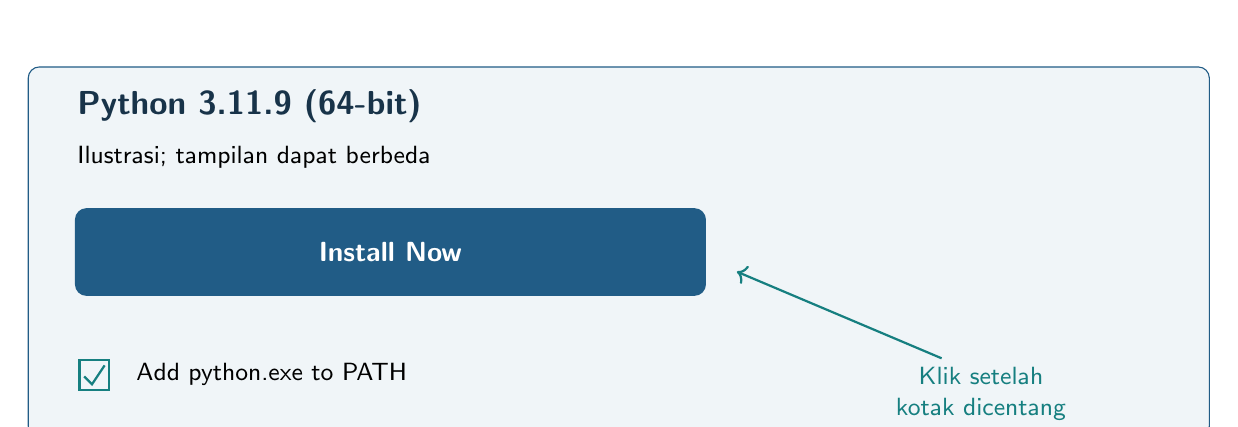
\begin{tikzpicture}
\draw[fill=pale,draw=blue,rounded corners] (0,0) rectangle (15,4.7);
\node[anchor=west,font=\bfseries\large,text=slate] at (0.5,4.2) {Python 3.11.9 (64-bit)};
\node[anchor=west,font=\small] at (0.5,3.55) {Ilustrasi; tampilan dapat berbeda};
\draw[fill=blue,draw=blue,rounded corners] (0.6,1.8) rectangle (8.6,2.9);
\node[text=white,font=\bfseries] at (4.6,2.35) {Install Now};
\draw[teal,thick] (0.65,0.6) rectangle (1.03,0.98);
\draw[teal,thick] (0.71,0.77)--(0.81,0.67)--(0.97,0.91);
\node[anchor=west,font=\small] at (1.25,0.8) {Add python.exe to PATH};
\draw[->,teal,thick] (11.6,1.0)--(9.0,2.1);
\node[text=teal,font=\small,align=center] at (12.1,0.55) {Klik setelah\\kotak dicentang};
\end{tikzpicture}\par
\step{3}{Selesaikan pemasangan}
Tunggu pesan sukses, klik \textbf{Close}, lalu tutup dan buka kembali terminal
yang sudah terbuka. Cara membuka PowerShell ada di halaman 4.
\begin{panel}{Mengapa versi ini?}
Panduan memakai jalur Python 3.11 yang diuji pada proyek. Rilis 3.11.9 dipilih
karena menyediakan installer Windows biasa. Ini \textbf{bukan klaim versi Python
terbaru}; rilis 3.11 yang lebih baru juga tersedia. Jangan mengganti versi utama
saat mengikuti langkah pertama kali.
\end{panel}
\source{1, 2}

\pagetitle{2}{Unduh proyek yang benar}{Ambil branch \textbf{development}, karena script hasil konversi berada pada branch ini.}
\step{1}{Buka GitHub}
Buka \href{https://github.com/ropok/grib-data-processing/tree/development}{halaman proyek pada branch development}.
Pastikan pilihan branch bertuliskan \textbf{development}, lalu klik
\textbf{Code} dan \textbf{Download ZIP}. Anda juga dapat memakai
\href{https://github.com/ropok/grib-data-processing/archive/refs/heads/development.zip}{tautan ZIP development langsung}.
\par\noindent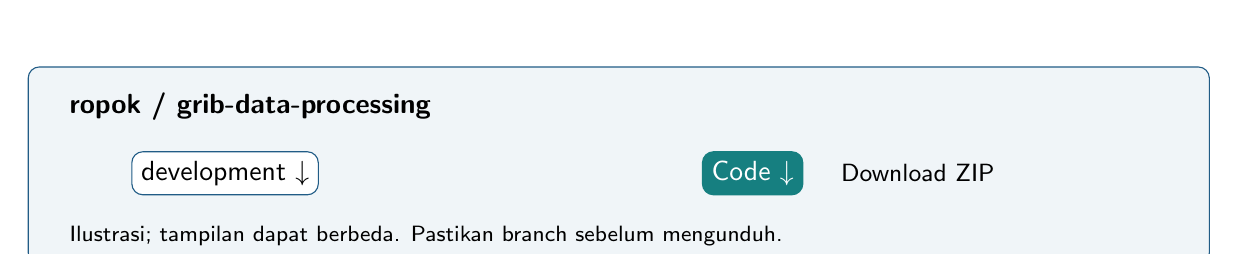
\begin{tikzpicture}
\draw[draw=blue,fill=pale,rounded corners] (0,0) rectangle (15,2.5);
\node[anchor=west,font=\bfseries] at (0.4,2.0) {ropok / grib-data-processing};
\node[draw=blue,rounded corners,fill=white] at (2.5,1.15) {development $\downarrow$};
\node[draw=teal,fill=teal,text=white,rounded corners] at (9.2,1.15) {Code $\downarrow$};
\node[anchor=west,font=\small] at (10.2,1.15) {Download ZIP};
\node[anchor=west,font=\footnotesize] at (0.4,0.35) {Ilustrasi; tampilan dapat berbeda. Pastikan branch sebelum mengunduh.};
\end{tikzpicture}\par
\step{2}{Ekstrak ZIP ke Documents}
Di File Explorer, klik kanan ZIP lalu pilih \textbf{Extract All / Ekstrak Semua}.
Buka folder hasil ekstraksi yang berisi script. Di bilah alamat Explorer,
masukkan lokasi berikut lalu tekan Enter:
\begin{terminal}
%USERPROFILE%\Documents
\end{terminal}
Pindahkan folder proyek ke sana, lalu ubah namanya menjadi
\code{grib-data-processing}. Jangan hanya membuka isi ZIP.
Jika Documents Anda dialihkan ke OneDrive, gunakan lokasi Documents yang
sebenarnya di Explorer. Salin alamat folder proyek itu untuk perintah
\code{cd "alamat folder proyek"} di halaman berikutnya.
\step{3}{Periksa isi folder proyek}
\begin{terminal}
Documents\grib-data-processing\
  grib_to_csv.py
  requirements.txt
  README.md
  AGENTS.md
  GribToCsv.ipynb
  tests\
\end{terminal}
\begin{panel}{Pastikan Anda berada pada folder yang tepat}
File \code{grib_to_csv.py} dan \code{requirements.txt} harus terlihat langsung
di folder proyek. Jika masih ada folder proyek di dalam folder proyek, buka
folder yang benar-benar berisi kedua file tersebut. GRIB diperoleh terpisah.
\end{panel}
\source{3, 4}

\pagetitle{3}{Buka PowerShell}{PowerShell adalah jendela untuk memberi perintah. Anda cukup menyalin baris yang disediakan.}
\step{1}{Buka terminal biasa}
Klik Start, ketik \textbf{PowerShell}, lalu buka \textbf{Windows PowerShell}.
Windows Terminal dengan tab PowerShell juga bisa dipakai. Tidak perlu memilih
\textbf{Run as administrator} untuk langkah proyek ini.
\step{2}{Masuk ke folder proyek}
Salin satu baris ini, tempel ke PowerShell, lalu tekan Enter:
\begin{terminal}
cd "$env:USERPROFILE\Documents\grib-data-processing"
\end{terminal}
\step{3}{Periksa folder dan Python}
Jalankan setiap baris berikut satu per satu:
\begin{terminal}
pwd
dir
py -3.11 --version
\end{terminal}
\begin{panel}{Tanda Anda siap melanjutkan}
\code{pwd} menampilkan lokasi folder proyek. \code{dir} menampilkan
\code{grib_to_csv.py} dan \code{requirements.txt}. Perintah terakhir menampilkan
\code{Python 3.11.x}. Jika tidak, lihat halaman 11 sebelum melanjutkan.
\end{panel}
\textbf{Cara membaca jendela terminal}\par
\par\noindent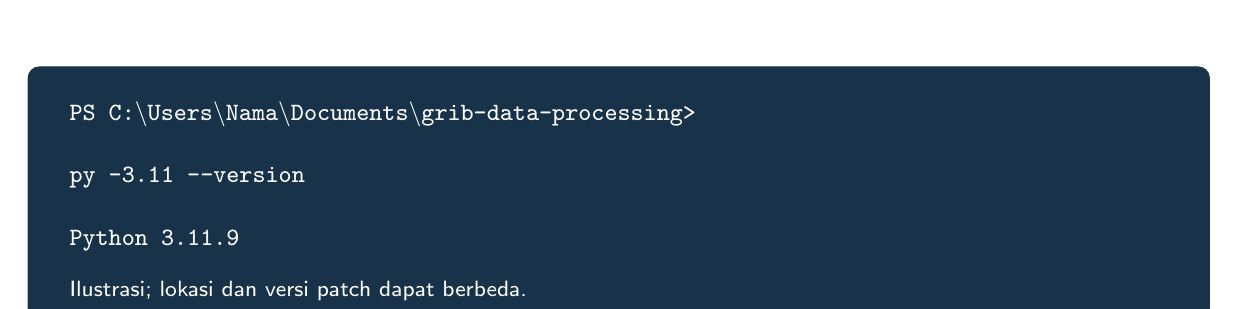
\begin{tikzpicture}
\draw[fill=slate,draw=slate,rounded corners] (0,0) rectangle (15,3.2);
\node[text=white,anchor=west,font=\ttfamily\small] at (0.4,2.6) {PS C:\textbackslash Users\textbackslash Nama\textbackslash Documents\textbackslash grib-data-processing>};
\node[text=white,anchor=west,font=\ttfamily\small] at (0.4,1.8) {py -3.11 -{}-version};
\node[text=white,anchor=west,font=\ttfamily\small] at (0.4,1.0) {Python 3.11.9};
\node[text=white,anchor=west,font=\footnotesize] at (0.4,0.35) {Ilustrasi; lokasi dan versi patch dapat berbeda.};
\end{tikzpicture}\par
Baris \code{PS ... >} adalah \textbf{prompt terminal}; jangan ikut menyalinnya.
Ketik hanya perintah. Tunggu sampai prompt muncul kembali sebelum menjalankan
perintah berikutnya. Teks lokasi hasil bisa berbeda menurut nama pengguna Anda.

\pagetitle{4}{Siapkan paket proyek}{Environment \code{.venv} menyimpan alat khusus untuk proyek ini. Buat sekali; setelah itu gunakan kembali.}
\step{1}{Buat environment}
Pastikan masih berada di folder proyek, lalu jalankan:
\begin{terminal}
py -3.11 -m venv .venv
\end{terminal}
Saat berhasil, biasanya tidak ada pesan khusus. Folder \code{.venv} akan dibuat.
\step{2}{Pasang dependensi}
\begin{terminal}
.\.venv\Scripts\python.exe -m pip install -r requirements.txt
\end{terminal}
Tunggu proses unduhan dan pemasangan selesai. Langkah ini membutuhkan internet.
Daftar paket dikunci dalam \code{requirements.txt} agar versi utama alat yang
dipakai sesuai dengan pengujian proyek. cfgrib/ecCodes membaca GRIB;
numpy/pandas/xarray mengolah data; openpyxl menulis Excel.
\step{3}{Periksa pemasangan}
\begin{terminal}
.\.venv\Scripts\python.exe -m pip check
\end{terminal}
Pesan yang diharapkan:
\begin{terminal}
No broken requirements found.
\end{terminal}
\begin{panel}{Tidak perlu aktivasi}
Perintah panduan langsung memakai Python di \code{.venv}. Anda tidak perlu
menjalankan \code{Activate.ps1}, mengubah execution policy, atau memasang paket
ke Python global.
\end{panel}
\par\noindent
\begin{tikzpicture}[node distance=7mm,>=Latex]
\node[draw=blue,fill=pale,rounded corners,text width=62mm,align=center,minimum height=19mm] (a) {\textbf{Python 3.11}\\Membuat environment};
\node[draw=teal,fill=pale,rounded corners,text width=62mm,align=center,minimum height=19mm,right=of a] (b) {\textbf{.venv}\\Menyimpan paket converter};
\draw[->,thick,teal] (a)--(b);
\end{tikzpicture}\par
\vfill
Jika ada tulisan \code{ERROR}, simpan seluruh pesan, termasuk perintah yang
Anda jalankan. Panduan masalah umum ada di halaman 11.

\pagetitle{5}{Masukkan data dan konversi}{Contoh berikut menggunakan nama sampel. Sesuaikan jika nama file Anda berbeda.}
\step{1}{Buat folder data}
Di File Explorer, buka folder proyek. Buat folder baru bernama \code{data}, lalu
salin file GRIB dari pemilik data ke dalamnya. Jika folder sudah ada, gunakan
folder tersebut.
\begin{terminal}
grib-data-processing\
  grib_to_csv.py
  data\
    PM 10 DAN PM 2,5 MENTAH.grib
\end{terminal}
\step{2}{Periksa nama file}
Di PowerShell pada folder proyek, jalankan:
\begin{terminal}
dir data\*.grib
\end{terminal}
Pastikan nama tampil sesuai. Aktifkan tampilan \textbf{File name extensions}
di Explorer jika perlu memastikan akhiran file; jangan menambahkan \code{.grib}
dua kali.
\step{3}{Jalankan konversi}
Jalankan dua baris ini secara berurutan. Baris pertama menyimpan path dalam
variabel \code{$inputFile}; tanda kutip melindungi nama yang mengandung spasi.
\begin{terminal}
$inputFile = "data\PM 10 DAN PM 2,5 MENTAH.grib"
.\.venv\Scripts\python.exe grib_to_csv.py $inputFile
\end{terminal}
\step{4}{Tunggu pesan sukses}
Untuk sampel proyek, pesan ringkasnya adalah:
\begin{terminal}
Exported 3168 rows; columns: year, month, day, hour, pm2p5, pm10
CSV: ...\PM 10 DAN PM 2,5 MENTAH.csv
XLSX: ...\PM 10 DAN PM 2,5 MENTAH.xlsx
\end{terminal}
\begin{panel}{Untuk penggunaan berikutnya}
Buka PowerShell, masuk lagi ke folder proyek (halaman 4), lalu ulangi langkah
di halaman ini untuk file baru. Environment tidak perlu dibuat ulang jika
masih tersedia. Jumlah baris dan variabel file Anda bisa berbeda.
\end{panel}

\pagetitle{6}{Temukan dan buka hasil}{CSV dan Excel berisi tabel yang sama. Folder hasil default berada di samping file input.}
\step{1}{Buka folder hasil di Explorer}
\begin{terminal}
data\
  PM 10 DAN PM 2,5 MENTAH.grib
  output_PM 10 DAN PM 2,5 MENTAH\
    PM 10 DAN PM 2,5 MENTAH.csv
    PM 10 DAN PM 2,5 MENTAH.xlsx
\end{terminal}
\step{2}{Buka Excel}
Klik dua kali file \code{.xlsx}. Jika Windows meminta aplikasi, pilih Excel
atau aplikasi spreadsheet yang mendukung XLSX. Baris pertama berisi nama kolom;
baris berikutnya berisi data. Jangan mengubah data mentah saat memeriksa hasil.
\vspace{2mm}
\begin{center}
\small\setlength{\tabcolsep}{7pt}
\begin{tabular}{rrrrll}
\toprule
\textbf{year}&\textbf{month}&\textbf{day}&\textbf{hour}&\textbf{pm2p5}&\textbf{pm10}\\
\midrule
2024&8&1&0&nilai GRIB&nilai GRIB\\
2024&8&1&3&nilai GRIB&nilai GRIB\\
\bottomrule
\end{tabular}\par
\footnotesize Ilustrasi susunan kolom; bukan angka konsentrasi contoh.
\end{center}
\step{3}{Pilih format yang sesuai}
XLSX paling mudah untuk melihat tabel di Excel. CSV adalah teks dengan pemisah
koma; bisa dibuka di editor teks atau diimpor melalui menu \textbf{Data / From
Text/CSV} pada aplikasi spreadsheet. Jika CSV tampak menjadi satu kolom, pilih
pemisah koma saat mengimpor. Anda juga bisa mengunggah hasil ke AI browser untuk
dibantu membaca tabel (halaman 10).
\par\textbf{Angka sangat kecil tetap dipertahankan.} Misalnya
\code{3.2129265e-08} berarti $3.2129265\times10^{-8}$, bukan error.
Periksa satuan aslinya sebelum menafsirkannya sebagai konsentrasi tertentu.

\begin{panel}{Hasil dengan nama sama akan ditulis ulang}
Salin hasil lama ke folder lain jika ingin menyimpannya sebelum mengulang
konversi. Tutup file XLSX yang sedang dibuka di Excel sebelum menjalankan ulang.
\end{panel}
\textbf{Opsional: pilih folder hasil yang lebih singkat}\par
Gunakan variabel \code{$inputFile} dari halaman sebelumnya:
\begin{terminal}
.\.venv\Scripts\python.exe grib_to_csv.py $inputFile --output-dir "data\hasil"
\end{terminal}
Salin seluruh perintah pada satu baris. Hasilnya disimpan dalam
\code{data\hasil} dengan nama file yang sama seperti contoh.

\pagetitle{7}{Pahami titik dan kolom waktu}{Konversi menjaga cara baca notebook. Memahami maknanya mencegah salah menafsirkan tabel.}
\textbf{Titik lokasi: koordinat terakhir pada kedua sumbu}\par
Script mengambil satu titik untuk tiap waktu, yaitu latitude terakhir dan
longitude terakhir. Ini bukan rata-rata seluruh wilayah. Pada sampel, titiknya
adalah latitude \textbf{-7.5}, longitude \textbf{111.0}.
\begin{center}
\par\noindent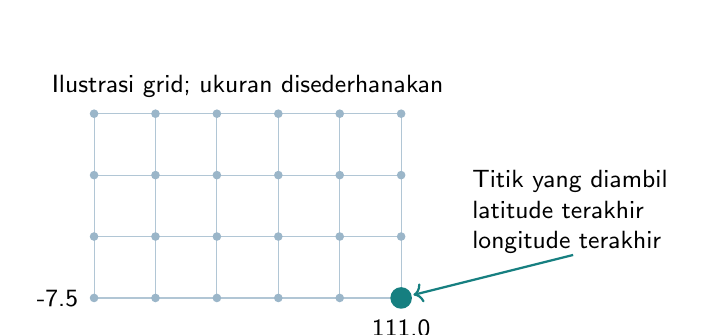
\begin{tikzpicture}[scale=0.78]
\draw[step=1,blue!35] (0,0) grid (5,3);
\foreach \x in {0,...,5} \foreach \y in {0,...,3} \fill[blue!45] (\x,\y) circle (2pt);
\fill[teal] (5,0) circle (5pt);
\draw[->,teal,thick] (7.8,0.7)--(5.2,0.05);
\node[align=left,anchor=west,font=\small] at (6,1.4) {Titik yang diambil\\latitude terakhir\\longitude terakhir};
\node[below,font=\small] at (5,-0.2) {111.0};
\node[left,font=\small] at (-0.1,0) {-7.5};
\node[above,font=\small] at (2.5,3.1) {Ilustrasi grid; ukuran disederhanakan};
\end{tikzpicture}\par
\end{center}
\begin{panel}{Dua jalur waktu yang didukung}
\textbf{Yearly}: dimensi waktu, latitude, longitude. Kolom tanggal dan
\code{hour} berasal dari timestamp referensi \code{time}.

\textbf{Monthly single}: dimensi waktu, step, latitude, longitude. Tanggal
tetap tanggal referensi; \code{hour} berisi durasi forecast \code{step} dalam
jam bulat. Pecahan jam dipotong mengikuti notebook.
\end{panel}
\begin{center}
\begin{tabular}{@{}lll@{}}
\toprule
\textbf{Contoh monthly}&\textbf{Hasil tabel}&\textbf{Artinya}\\
\midrule
time: 1 Jan 2025&year=2025, month=1, day=1&Tanggal referensi\\
step: 27 jam&hour=27&Durasi, bukan jam harian\\
\bottomrule
\end{tabular}\par
\end{center}
Script tidak mengganti tanggal menjadi tanggal \code{valid_time}. Jangan
menganggap \code{hour=27} sebagai kesalahan atau mengubahnya ke jam 03 sendiri.
Satuan variabel dan zona waktu harus diperiksa dari metadata GRIB atau pemilik
data; jangan menganggap semua data memakai satuan tertentu atau WIB.
Sampel lokal memiliki jalur yearly; monthly sejauh ini diuji dengan data sintetis.

\pagetitle{8}{Minta Codex mengerjakan lokal}{Codex desktop dapat membantu di folder proyek yang Anda pilih, sesuai akses dan persetujuan sesi.}
\step{1}{Pasang dan masuk ke aplikasi}
Buka \href{https://learn.chatgpt.com/docs/windows/windows-app}{panduan aplikasi Windows resmi}.
Gunakan tautan Microsoft Store pada panduan tersebut untuk mengunduh aplikasi,
lalu masuk dengan akun Anda. Ketersediaan dan tampilan aplikasi bisa berubah.
Ikuti petunjuk resmi jika nama menu berbeda.
\step{2}{Pilih Codex dan folder proyek}
Di aplikasi, pilih pengalaman \textbf{Codex}. Buka atau pilih folder lokal
\code{Documents\grib-data-processing} melalui pemilih folder. Pastikan folder
yang dipilih berisi script, \code{README.md}, dan \code{AGENTS.md}.
\step{3}{Kirim prompt lengkap}
\begin{panel}{Prompt siap pakai}
Saya bukan programmer. Baca AGENTS.md dan README.md di proyek ini. Tolong
konversi file "data/PM 10 DAN PM 2,5 MENTAH.grib" menjadi CSV dan Excel.
Gunakan Python 3.11 dan environment .venv; siapkan paket jika belum ada.
Ikuti aturan model: GPT 6 Astra medium untuk planning dan GPT 6.1 Sol high
untuk pelaksanaan. Jika tidak tersedia, laporkan dan jangan mengganti
model diam-diam. Pertahankan file asli. Jalankan prosesnya, lalu beri lokasi
hasil, jumlah baris, variabel, serta arti titik dan kolom waktunya.
\end{panel}
\step{4}{Periksa jawaban dan persetujuan akses}
AI mungkin perlu persetujuan untuk mengunduh paket atau menulis pada folder
tertentu. Baca tujuan tindakannya. Setelah selesai, buka hasil di folder yang
dilaporkan dan cocokkan jumlah baris/kolom dengan laporan.
\begin{panel}{Aturan model perlu konfigurasi nyata}
Tulisan dalam AGENTS.md tidak otomatis mengganti model aplikasi. Pilih model
dan reasoning effort yang tersedia pada pengaturan sesi atau agent. Jika
pilihan yang diminta tidak tersedia, minta AI menjelaskan keterbatasannya.
Script converter sendiri tidak membutuhkan login OpenAI atau API key.
\end{panel}
\source{5, 6}

\pagetitle{9}{Gunakan AI lewat browser}{AI browser membantu menjelaskan perintah dan membaca file yang Anda unggah. Path lokal saja tidak memberikan akses ke file.}
\step{1}{Buka percakapan}
Buka \href{https://chatgpt.com}{chatgpt.com} di browser, masuk, lalu buat chat.
Sertakan README atau AGENTS yang Anda salin/unggah agar konteks proyek jelas.
\step{2}{Minta panduan menjalankan di komputer Anda}
\begin{panel}{Prompt pendamping PowerShell}
Saya pengguna Windows nonprogrammer. Proyek saya ada di
Documents/grib-data-processing dan file input bernama
"data/PM 10 DAN PM 2,5 MENTAH.grib". Bantu saya menjalankan converter lokal
dengan Python 3.11 dan .venv berdasarkan README yang saya berikan.
Beri satu langkah setiap kali, jelaskan hasil yang seharusnya tampil,
dan tunggu laporan saya sebelum langkah berikutnya. Jangan menganggap
Anda dapat membaca file lokal saya dari nama path saja.
\end{panel}
Jika terjadi error, kirim perintah yang dijalankan dan teks error lengkap.
Anda tetap menjalankan perintah pada PowerShell sendiri.
\step{3}{Unggah hasil untuk dibantu membacanya}
Gunakan tombol lampiran untuk mengunggah CSV atau XLSX jika fitur tersedia,
lalu kirim prompt berikut:
\begin{panel}{Prompt pemeriksaan hasil}
Periksa file tabel yang saya unggah. Laporkan nama kolom, jumlah baris data,
nilai kosong, dan rentang tanggal. Jangan menebak satuan atau zona waktu.
Jelaskan bahwa converter mengambil titik terakhir latitude/longitude;
untuk monthly, hour adalah durasi step, bukan jam \code{valid_time}.
Jika file tidak dapat dibaca, jelaskan apa yang perlu saya berikan.
\end{panel}
\begin{panel}{Bisakah browser langsung mengonversi GRIB?}
Hanya jika sesi mendukung unggahan file tersebut \emph{dan} lingkungan
eksekusinya menyediakan dependensi GRIB yang diperlukan. Ini tidak dijamin.
Menulis \code{C:\...} atau \code{D:\...} dalam chat tidak membuka file komputer
Anda. Jika tidak didukung, jalankan script secara lokal dan unggah hasilnya.
\end{panel}
\source{7, 8}

\pagetitle{10}{Jika ada masalah}{Mulai dari pesan yang terlihat. Jangan menghapus data atau memasang ulang semuanya sebagai langkah pertama.}
\begin{tabular}{@{}p{49mm}p{108mm}@{}}
\toprule
\textbf{Pesan / keadaan}&\textbf{Yang dilakukan}\\
\midrule
\code{py} tidak dikenali&Periksa Python 3.11 sudah terpasang; buka terminal baru. Jika launcher tidak tersedia, gunakan path Python pada kotak di bawah.\\[6pt]
Script atau requirements tidak ditemukan&Ulangi \code{cd} pada halaman 4; jalankan \code{dir}. Pastikan script langsung berada di folder itu, bukan dalam ZIP atau folder bertingkat.\\[6pt]
Input file does not exist&Jalankan \code{dir data\*.grib}. Cocokkan nama, akhiran, spasi, dan path dalam tanda kutip.\\[6pt]
\code{pip} gagal mengunduh&Periksa internet dan pesan proxy/firewall. Kirim error lengkap kepada AI/pendamping. Setelah penyebab diperbaiki, ulangi instalasi requirements.\\[6pt]
Permission denied pada XLSX&Tutup file hasil di Excel. Jika folder tidak dapat ditulis, gunakan \code{--output-dir "data\hasil"}.\\[6pt]
GRIB memerlukan filter / unsupported dimensions&Kirim pesan lengkap ke AI. Minta pemeriksaan kunci GRIB dan dimensi; jangan menebak filter atau mengubah data.\\
\bottomrule
\end{tabular}\par
\vspace{3mm}
\textbf{Alternatif membuat environment jika launcher tidak tersedia}\par
Untuk pemasangan per pengguna pada lokasi bawaan Python 3.11, jalankan:
\begin{terminal}
$python = "$env:LOCALAPPDATA\Programs\Python\Python311\python.exe"
& $python -m venv .venv
\end{terminal}
Jika file ini juga tidak ditemukan, periksa lokasi Python yang sebenarnya;
path tersebut hanya berlaku untuk lokasi pemasangan bawaan.
\begin{panel}{Prompt diagnosis yang membantu}
Saya menjalankan perintah berikut: [tempel perintah]. Pesannya: [tempel
error lengkap]. Lokasi proyek: [hasil pwd]. Isi folder: [hasil dir].
Tolong jelaskan penyebab yang dapat diperiksa dan beri satu langkah perbaikan
pada satu waktu. Pertahankan data asli; jangan menebak filter GRIB.
\end{panel}
\source{2}

\pagetitle{11}{Periksa sebelum selesai}{Simpan file asli, hasil, dan catatan pemeriksaan agar proses bisa diulangi.}
\begin{itemize}
\item File CSV dan XLSX tersedia; nama dan foldernya sesuai input yang dipilih.
\item Nama kolom, jumlah baris, titik grid, dan arti waktu dipahami.
\item Hasil lama disalin jika perlu disimpan sebelum konversi berikutnya.
\item Sampel yang diuji menghasilkan 3.168 baris data dan enam kolom;
      monthly baru memiliki bukti pengujian sintetis.
\end{itemize}
\begin{panel}{Prompt verifikasi dengan Codex lokal}
Tolong buktikan hasil script sama dengan notebook asli pada sampel dalam data.
Jalankan pengujian parity yang tersedia dan pip check. Jelaskan perbandingan
DataFrame, normalisasi akhir baris CSV, isi/style Excel, mana yang memakai
GRIB asli, dan lokasi laporannya. Jangan mengubah notebook atau data mentah.
\end{panel}
\textbf{Bacaan resmi dan sumber proyek}\par
\small
Tautan diperiksa pada \textbf{13 Oktober 2026}. Nomor sumber dipakai dekat
petunjuk terkait; isi teknis converter berasal dari README dan script proyek.
\begin{enumerate}[label={[\arabic*]},leftmargin=7mm,itemsep=2pt]
\item \href{https://www.python.org/downloads/release/python-3119/}{Python 3.11.9: unduhan dan Windows installer (64-bit).}
\item \href{https://docs.python.org/3.11/using/windows.html}{Python 3.11: panduan pemasangan dan launcher Windows.}
\item \href{https://github.com/ropok/grib-data-processing/tree/development}{Proyek: branch development, README, AGENTS, dan script.}
\item \href{https://docs.github.com/en/repositories/working-with-files/using-files/downloading-source-code-archives}{GitHub: mengunduh arsip source code.}
\item \href{https://learn.chatgpt.com/docs/windows/windows-app}{OpenAI: aplikasi Windows dan tautan unduhan resmi.}
\item \href{https://learn.chatgpt.com/docs/app}{OpenAI: penggunaan aplikasi dan Codex.}
\item \href{https://learn.chatgpt.com/docs/web}{OpenAI: penggunaan ChatGPT di web.}
\item \href{https://learn.chatgpt.com/docs/use-chatgpt}{OpenAI: cara memakai ChatGPT dalam berbagai lingkungan.}
\end{enumerate}
\normalsize
\textbf{Untuk pengelola dokumentasi}\par
Sumber panduan ini adalah \code{docs/panduan-pengguna.tex}; PDF dibangun dari
sumber yang sama. Petunjuk rebuild ada di \code{docs/README.md}. Pengguna
converter tidak perlu memasang LaTeX untuk mengikuti panduan.
\end{document}
